\documentclass[11pt]{article}
\usepackage[utf8]{inputenc}
\usepackage{graphicx}
\usepackage{listings}
\usepackage{geometry}
\usepackage{hyperref}
\usepackage{dirtree}
\usepackage{float}

\geometry{a4paper, margin=1in}

\title{Verification of a Configurable Vending Machine Controller}
\author{Reza}
\date{\today}

\begin{document}

\maketitle
\tableofcontents
\newpage

\section{Verification Environment and Reproducibility}
For making development and test, I have tried to create an Environment based on Docker image that is combination of configuration of vsim and HARM tools. The tools is available on a Github repository.
\begin{center}
    \url{https://github.com/MrzAhmadi/SVT-Environment}
\end{center}

\section{Project files hierarchy}
\begin{figure}[h]
    \centering
    \begin{minipage}{0.6\textwidth} % Adjust width as needed
        \dirtree{%
            .1 /.
            .2 1\_rtl.
            .3 vending\_machine.sv.
            .2 2\_simple\_tb.
            .3 simple\_tb.sv.
            .2 3\_random\_tb.
            .3 random\_tb.sv.
            .2 4\_assertions.
            .3 assertions.sv.
            .3 bind.sv.
            .2 5\_harm.
            .3 conf.xml.
            .3 mined\_assertions.txt.
            .2 6\_traces.
            .3 assertions.vcd.
            .3 random\_tb.vcd.
            .3 simple\_tb.vcd.
            .2 7\_scripts.
            .3 run\_assertions.sh.
            .3 run\_harm.sh.
            .3 run\_random.sh.
            .3 run\_simple.sh.
            .2 8\_report.
            .3 report.pdf.
            .3 report.tex.
        }
    \end{minipage}
    \caption{Project Directory Structure}
    \label{fig:dir_structure}
\end{figure}

\section{System Specifications and Design (Part 1)}
% Goal: Address Part 1.1 requirements
\subsection{RTL Implementation and FSM Logic}

The main purpose of this section is design a finite state machine (FSM) to manage the vending machine lifecycle. The main design file is located at \texttt{/1\_rtl/vending\_machine.sv}. This implementation covers all demanded features of vending machine in the part of 1.1 of assignment.

\subsubsection*{State Transition Table}
The following table describes the behavior of the FSM across its three primary states:

\begin{table}[h!]
\centering
\renewcommand{\arraystretch}{1.5}
\begin{tabular}{|l|l|p{6cm}|}
\hline
\textbf{Current State} & \textbf{Next State} & \textbf{Condition / Action} \\ \hline
\textbf{IDLE} & \textbf{IDLE} & Accumulating credit via \texttt{coin\_in}. Valid coins: 10, 20, 50, 100, 200. \\ \hline
\textbf{IDLE} & \textbf{DELIVER} & \texttt{button\_in} pressed AND \texttt{credit} $\ge$ cost (30 for Water, 50 for Soda). Subtract cost from credit. \\ \hline
\textbf{DELIVER} & \textbf{CHANGE} & Timer reaching $N$ cycles. Assert \texttt{beverage\_out}. Transition if \texttt{credit} > 0 and cannot buy more items. \\ \hline
\textbf{DELIVER} & \textbf{IDLE} & Timer reaching $N$ cycles. Assert \texttt{beverage\_out}. Transition if \texttt{credit} == 0. \\ \hline
\textbf{CHANGE} & \textbf{IDLE} & Timer reaching $M$ cycles. Assert \texttt{change\_out} and reset credit to 0. \\ \hline
\end{tabular}
\caption{FSM State transitions and associated logic for the Vending Machine.}
\end{table}

\subsection{Functional Testing (Simple Testbench)}
In this part we describe the manual test cases from Part 1.2 of assignment. The file that is located at \url{2_simple_tb/simple_tb.sv}. In this simple testbench we consider some scenarios to test on our FSM vending machine.
First of all we initialize system in 20ns period then we try to test some cases in this order:
\begin{itemize}
    \item Water Purchase (Exact Change): Inserts 30 cents (10 + 20) and select water (button1)
    \item Water Delivery Timing: Trying to verify N cycles after press the button
    \item Soda Purchase (with Change): Inserts 60 cents (50 + 10) and select soda (button2)
    \item Change Return Logic: Confirming that machine returns remaining 10 cents
    \item Change Return Timing: Trying to verify M cycles after delivery.
\end{itemize}
For running this test bench, we have dedicated a bash script that is located at \url{7_scripts/run_simple.sh}. This script compiles the vending\_machine FSM and the simple testbench using \texttt{vlog}, and then runs \texttt{vsim} to create traces and save them at \url{6\_traces/simple\_tb.vcd}.

\begin{figure}[H]
    \centering
    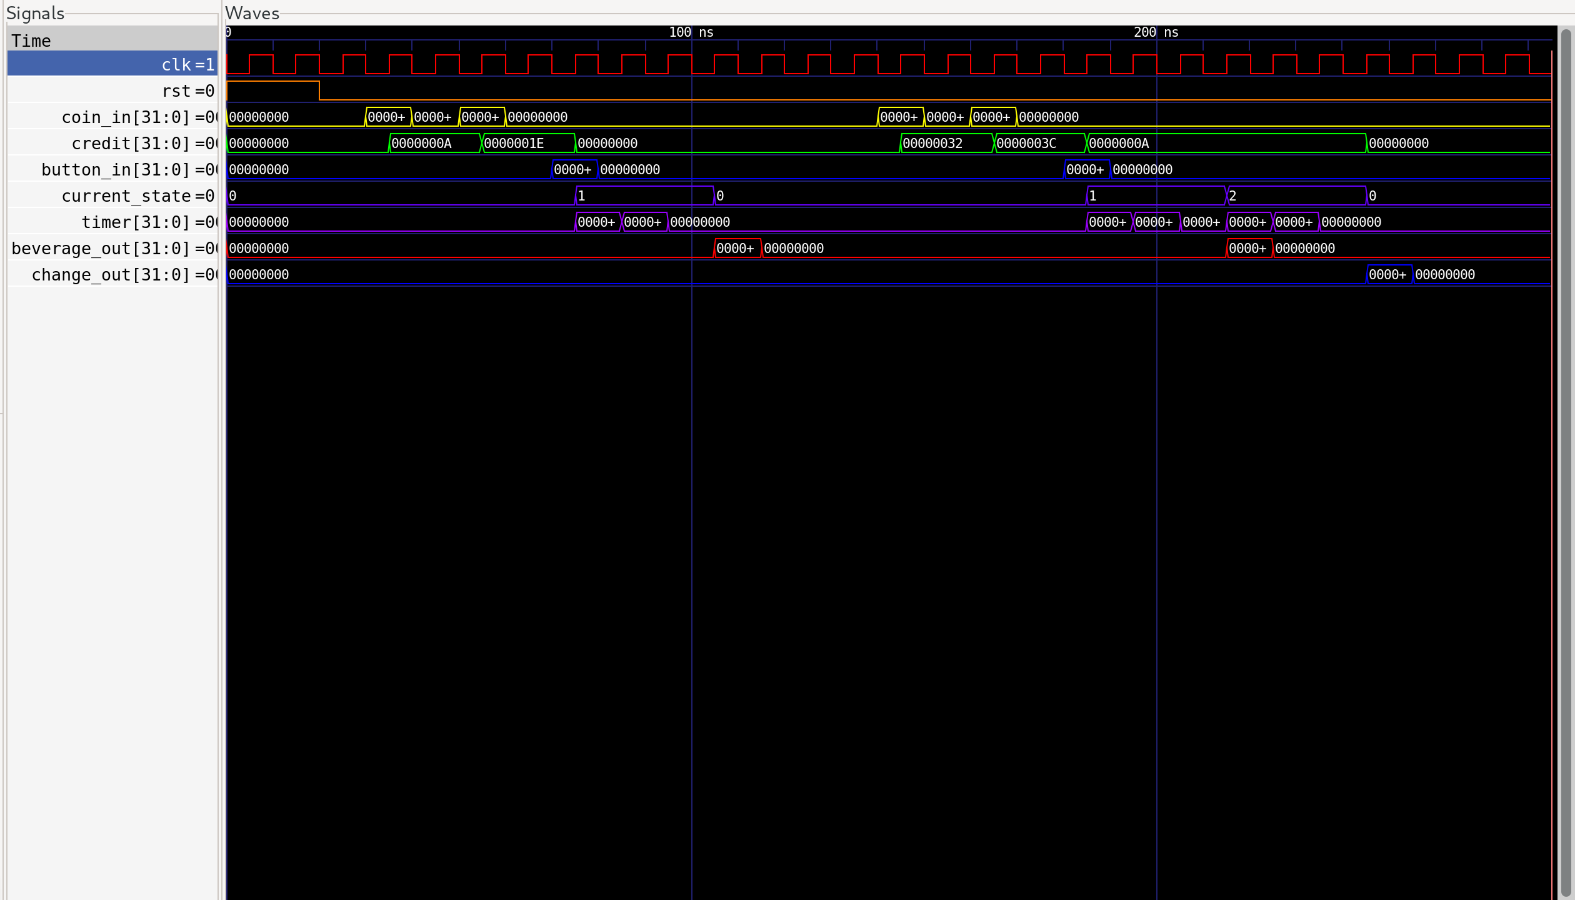
\includegraphics[width=1.0\textwidth]{screenshot_simple.png}
    \caption{Simulation trace of the simple testbench (Part 1.2). The waveform demonstrates a successful Water purchase (0-120ns) followed by a Soda purchase with change return (150-280ns), confirming the FSM transitions and $N$/$M$ cycle delays.}
    \label{fig:simple_tb}
\end{figure}

\subsection{Constrained Random Verification}
This is an implementation for Part 1.3. The random testbench is located at \url{random_tb/random_tb.sv}. It uses a generator and a transition class automatically create 2,000 cycles of test data. There were some efforts to apply realistic distribution to mimic real-world human. There are some implementation for HARM mining. There is also another bash script at \url{7_scripts/run_random.sh} that runs this random testbench and saves traces at \url{6_traces/random_tb.vcd}.

\begin{figure}[H]
    \centering
    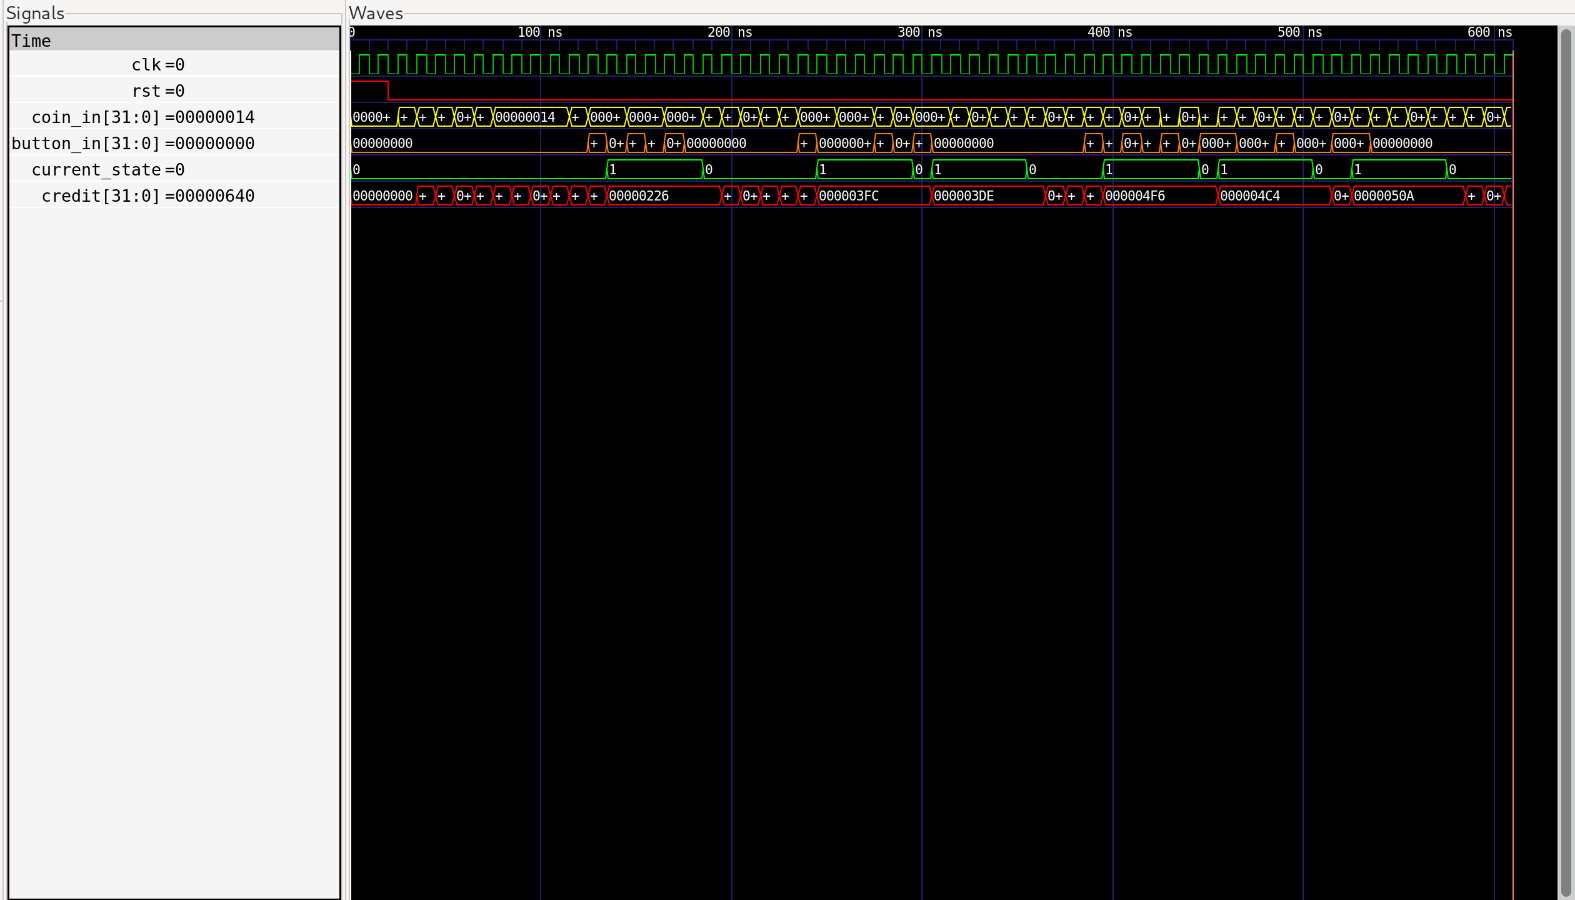
\includegraphics[width=1.0\textwidth]{screenshot_random.png}
    \caption{Trace of the Constrained Random Testbench (Part 1.3). The simulation drives the design with randomized coin inputs, resulting in high credit accumulation (e.g., reaching 0x226 or 550 cents) and frequent state transitions. The design remains stable and correctly returns to the IDLE state (0) after each transaction.}
    \label{fig:random_trace}
\end{figure}

\section{Assertion-Based Verification (Part 2)}
This section covers the implementation of formal checks to verify the temporal behavior of the design. The assertions are located in the \texttt{4\_assertions/} directory.

\begin{figure}[H]
    \centering
    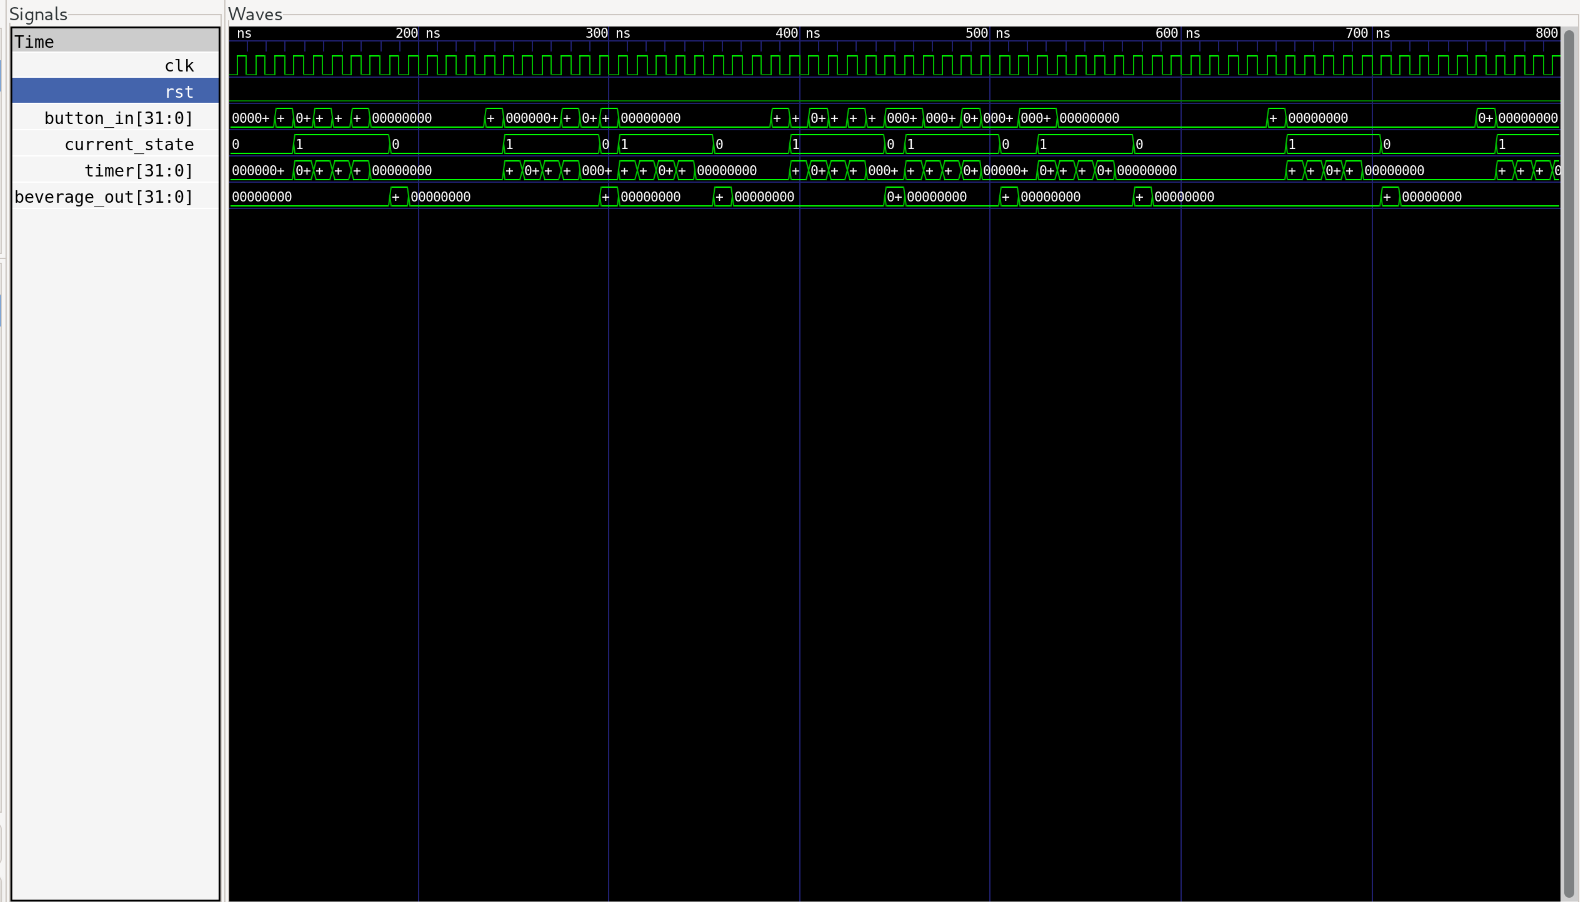
\includegraphics[width=1.0\textwidth]{screenshot_assertion_1.png}
    \caption{Visual verification of the \texttt{a\_water\_delivery} assertion over multiple transactions. The waveform confirms that every time the FSM enters the DELIVER state (1), the timer counts correctly, and the beverage output is asserted after the delay, verifying the property holds consistently.}
    \label{fig:assertion_multiple}
\end{figure}

\begin{figure}[H]
    \centering
    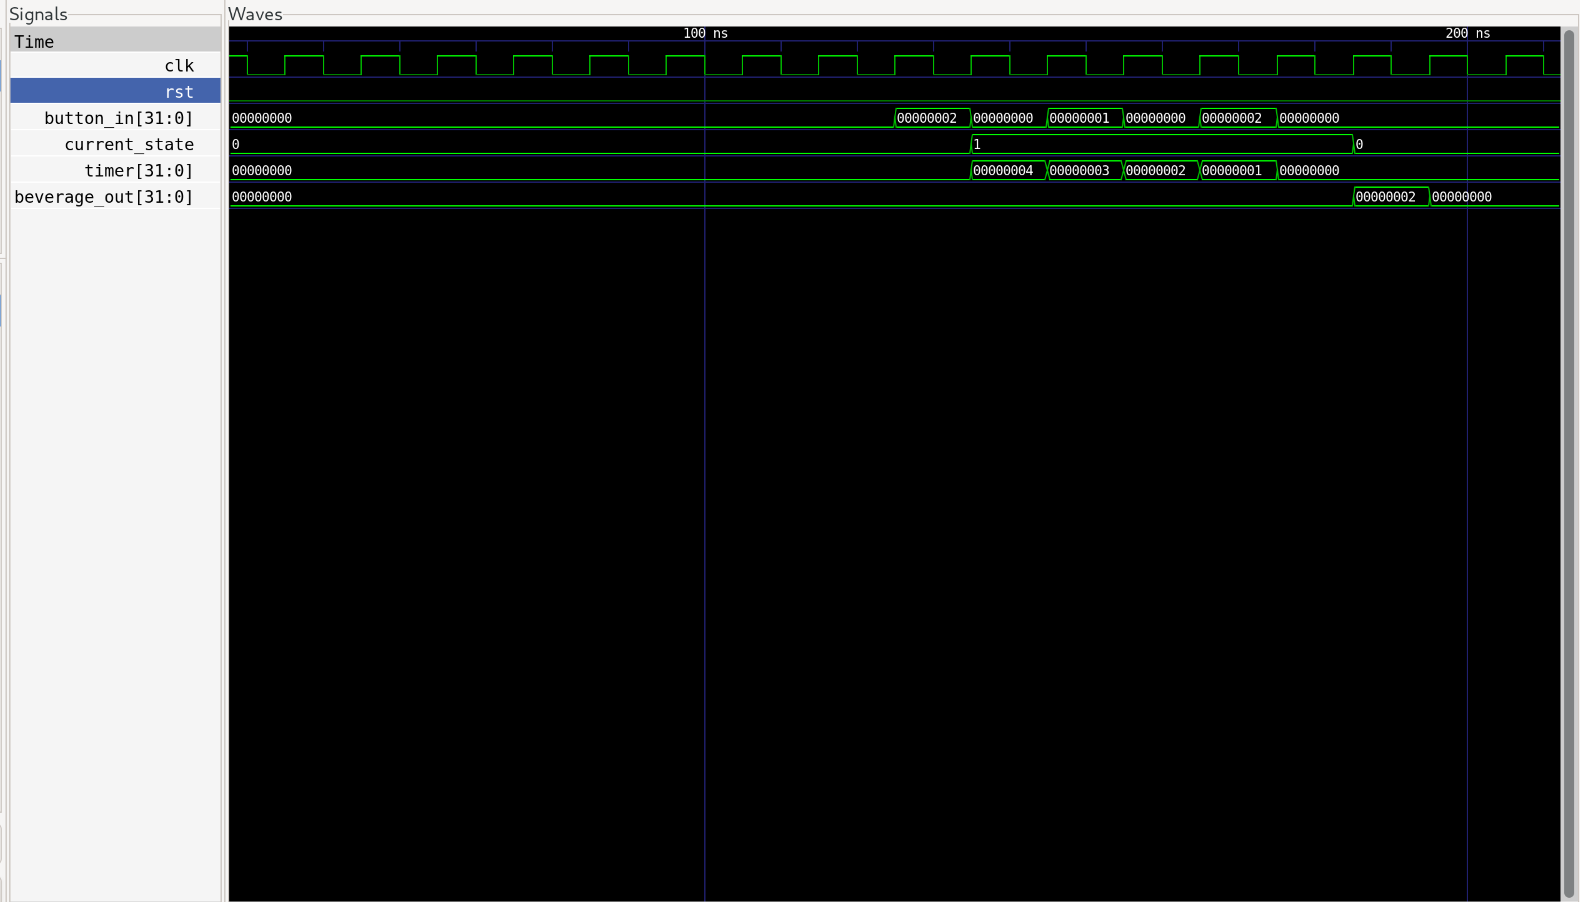
\includegraphics[width=1.0\textwidth]{screenshot_assertion_2.png}
    \caption{Detailed visual verification of the \texttt{a\_soda\_delivery} assertion. The trace shows a Soda request (\texttt{button\_in}=2), followed by the \texttt{timer} counting down exactly $N=4$ cycles while in the DELIVER state (1), before asserting \texttt{beverage\_out}.}
    \label{fig:assertion_detail}
\end{figure}

\subsection{Temporal Property Definitions}
For Part 2.1, five temporal assertions were developed in SystemVerilog (SVA) within the \texttt{vending\_props.sv} file. These properties monitor the FSM:

\begin{itemize}
    \item \textbf{Reset Safety (\texttt{a\_reset})}: Verifies that when the reset signal is high, the internal credit, beverage output, and change output are all forced to zero.
    \item \textbf{Credit Integrity (\texttt{a\_coin\_inc})}: Ensures that in the IDLE state, the credit register correctly increments using the \texttt{\$past} function.
    \item \textbf{Water Delivery Timing (\texttt{a\_water\_delivery})}: Checks that beverage output is asserted exactly $N$ clock cycles later.
\end{itemize}

\subsection{Checker Binding and Simulation}
A separate file \texttt{4\_assertions/bind.sv} was created to attach the \texttt{vending\_props} checker to the \texttt{vending\_machine} module. 

To run this simulation, the script \texttt{7\_scripts/run\_assertions.sh} is used. This script compiles the design and executes the simulation with the \texttt{-assertdebug} flag then we run another bash script at \url{7_scripts/run_harm.sh} At the end it saves traces at \url{6_traces/assertions.vcd}.

\section{Assertion Mining (Part 3)}
The HARM tool was used to automatically discover design properties from the execution traces.

\subsection{Configuration and Results}
The \texttt{conf.xml} defines manual templates for delivery timing and uses numeric clustering to identify signal patterns. HARM analyzed 2,000 cycles of data and successfully mined the FSM logic, which is documented in \texttt{5\_harm/mined\_assertions.txt}. These results confirm that the design satisfies the temporal requirements discovered during simulation.



\subsection{Mining Results and Correlation}

\begin{table}[h!]
\centering
\scriptsize
\renewcommand{\arraystretch}{1.3} % Adds a little breathing room between rows
\setlength{\tabcolsep}{4pt} % Adjusts column padding to fit page better
\begin{tabular}{|c|l|c|c|c|}
\hline
\textbf{N} & \textbf{Assertion (Context : default)} & \textbf{final} & \textbf{causality} & \textbf{frequency} \\ \hline
0 & \texttt{G(\{!(harm\_bev==32'b1) \&\& !(harm\_bev==32'b10)\} \textbar-> harm\_bev==32'b0)} & 1.00 & 1.00 & 1.00 \\ \hline
1 & \texttt{G(\{!(harm\_btn==32'b1) \&\& !(harm\_btn==32'b10)\} \textbar-> harm\_btn==32'b0)} & 1.00 & 1.00 & 0.90 \\ \hline
2 & \texttt{G(\{!(harm\_btn==32'b0) \&\& !(harm\_btn==32'b10)\} \textbar-> harm\_btn==32'b1)} & 0.00 & 1.00 & 0.11 \\ \hline
3 & \texttt{G(\{!(harm\_btn==32'b0) \&\& !(harm\_btn==32'b1)\} \textbar-> harm\_btn==32'b10)} & 0.00 & 1.00 & 0.10 \\ \hline
4 & \texttt{G(\{!(harm\_bev==32'b0) \&\& !(harm\_bev==32'b10)\} \textbar-> harm\_bev==32'b1)} & 0.00 & 1.00 & 0.06 \\ \hline
5 & \texttt{G(\{!(harm\_bev==32'b0) \&\& !(harm\_bev==32'b1)\} \textbar-> harm\_bev==32'b10)} & 0.00 & 1.00 & 0.05 \\ \hline
6 & \texttt{G(\{!(harm\_bev==32'b0) \#\#3 true\} \textbar-> harm\_bev==32'b0)} & 0.00 & 0.09 & 0.10 \\ \hline
10 & \texttt{G(\{rst \#\#4 true\} \textbar-> harm\_btn==32'b0)} & 0.00 & 0.19 & 0.00 \\ \hline
12 & \texttt{G(\{rst\} \textbar-> harm\_btn==32'b0)} & 0.00 & 0.19 & 0.00 \\ \hline
15 & \texttt{G(\{harm\_bev==32'b1 \#\#4 true\} \textbar-> harm\_bev==32'b0)} & 0.00 & 0.09 & 0.06 \\ \hline
24 & \texttt{G(\{rst\} \textbar-> harm\_bev==32'b0)} & 0.00 & 0.09 & 0.00 \\ \hline
\end{tabular}
\caption{Mined assertions from HARM output.}
\label{tab:harm_results}
\end{table}

\end{document}